\documentclass[11pt]{article}

\usepackage[margin=1in]{geometry}
\usepackage{amsmath}
\usepackage{algorithm}
\usepackage{algpseudocode}
\usepackage{booktabs}
\usepackage{hyperref}
\usepackage{xcolor}
\usepackage{tikz}
\usetikzlibrary{arrows.meta,positioning}

\definecolor{junaBlue}{HTML}{1F4E79}
\definecolor{junaGreen}{HTML}{2E7D32}
\definecolor{junaGold}{HTML}{8A5A00}
\definecolor{softPanel}{HTML}{F5F8FA}

\newcommand{\code}[1]{\texttt{#1}}
\newcommand{\juna}{JUNA}

\title{\juna{} for Newcomers: A Runnable Path from OFDM to a Code-Aware Receiver}
\author{A guided note based on the local \code{Juna/} package}
\date{\today}

\begin{document}
\maketitle

\begin{abstract}
This note explains \juna{} as a learning object rather than as a benchmark
paper. The central idea is simple: ordinary OFDM treats equalization and error
correction as separate stages, while \juna{} lets the decoder feed useful
confidence information back into the equalizer. The local package makes this
idea teachable because the transmitter, receiver, and their LDPC, partial-FFT,
and Doppler-sync internals sit behind one small interface: \code{init},
\code{modulate}, and \code{demodulate}. After a one-time setup
(environment plus the external LDPC build tools), a newcomer can run one file,
\code{demo\_isi\_ici\_awgn.jl}, and see a frame pass through multipath, Doppler,
and AWGN with zero post-FEC bit errors in the tested realization.
\end{abstract}

\section{Why Another \juna{} Paper?}

The journal paper answers a research question: when does a code-aware receiver
improve measured underwater acoustic OFDM? A newcomer usually asks a different
question: what is \juna{} doing, where does the code enter, and how can I run the
smallest example without learning the whole research stack first?

This folder suggests a better beginner story. It contains:
\begin{itemize}
  \item a single runnable demo, \code{demo\_isi\_ici\_awgn.jl};
  \item a shared modulation interface, \code{Modulations.jl};
  \item the implementation, \code{Juna.jl};
  \item an LDPC wrapper, \code{LDPC.jl};
  \item a reference write-up, \code{juna\_doc.pdf};
  \item a UnetStack/Yoda fit study in \code{bench/}, where Yoda
        (\code{org.arl.yoda}) is the software-defined-modem PHY that provides
        the usual PHYSICAL/BASEBAND layer on UnetStack/Subnero modems.
\end{itemize}

Those pieces make a natural learning ladder, and this note climbs it: start
with the interface, run one channel demo, then reveal why the decoder can help
the equalizer. Each section below is one rung.

\section{The One-Sentence Model}

\begin{quote}
\juna{} is coded OFDM with a partial-FFT equalizer and an LDPC decoder that
feeds soft information back to the equalizer when Doppler smears each tone's
energy into its neighbours.
\end{quote}

The main terms are:
\begin{center}
\begin{tabular}{p{0.14\linewidth}p{0.76\linewidth}}
\toprule
Term & In one line \\
\midrule
OFDM & Orthogonal frequency-division multiplexing: send bits on many parallel tones. \\
CP & Cyclic prefix: a guard copy prepended to each OFDM symbol to absorb echoes. \\
pilot & A known symbol used to measure the channel; \juna{} uses comb-type pilots across tones. \\
partial-FFT view & One receiver-side windowed FFT observation: samples from one short-time window of an OFDM symbol are kept, the rest is zeroed, and an \(N\)-point FFT is taken. Older code may index this as a branch, but it is not an antenna, propagation path, or delay tap. \\
short-time window & The contiguous interval inside one CP-removed OFDM symbol used to form one partial-FFT view. \\
ISI & Inter-symbol interference: neighbouring OFDM symbols bleeding into one another. \\
ICI & Inter-carrier interference: tones bleeding into one another. \\
AWGN & Additive white Gaussian noise: an idealized flat Gaussian noise floor; real ocean ambient noise is colored and non-Gaussian. \\
LDPC & Low-density parity-check: the error-correcting code \juna{} decodes. \\
BP & Belief propagation; \juna{} uses a normalized min-sum approximation that also yields per-bit confidence. \\
LLR/logit & Signed soft bit reliability. In robust mode, \(z\) is an LLR-like bit coordinate and \(\tanh(z/2)\) is the corresponding soft bit value. \\
soft & Confidence-carrying, not just hard 0/1; unsure values shrink toward zero. \\
posterior & Post-decoding belief about a bit or symbol after LDPC uses the parity checks. \\
RLS/LS fit & The ridge-regularized least-squares fit used by the partial-FFT combiner; the code labels this path RLS, but it is not the recursive-LS algorithm. \\
CFO & Carrier-frequency offset. Here Doppler is a wideband time-scale \(a\); \juna{} reports it in the CFO slot as \(\mathrm{cfo}\approx(a-1)f_c\), the offset at the carrier. \\
\bottomrule
\end{tabular}
\end{center}

That sentence has four parts:
\begin{enumerate}
  \item OFDM carries bits on many frequency tones. Here, an OFDM symbol means
        one CP-protected transform block.
  \item Multipath and Doppler stress the frame in different ways, and it helps
        to keep them apart. Multipath delay spread that fits inside the cyclic
        prefix leaves the tones separable; each tone mainly receives a complex
        gain. Echoes that overrun the CP spill across OFDM-symbol boundaries as
        inter-symbol interference. Doppler time-scales the whole waveform,
        which breaks subcarrier orthogonality and leaks tone energy between
        neighbours. The chirp sync removes the bulk time-scale; \juna{} targets
        the residual ICI left within each OFDM symbol.
  \item Partial FFTs give several time-windowed views of each tone.
  \item The LDPC decoder says which tentative symbols are trustworthy enough to
        reuse as soft training anchors.
\end{enumerate}

\section{The Small Interface That Makes It Learnable}

The most beginner-friendly part of the package is not a specific equation. It is
the interface in \code{Modulations.jl}. A modem object is expected to implement
the same small contract:

\begin{center}
\begin{tabular}{p{0.34\linewidth}p{0.28\linewidth}p{0.28\linewidth}}
\toprule
Function & Input idea & Output idea \\
\midrule
\code{init(m, fc, fs)} & modem plus carrier/sample rates & reset defaults, prep state \\
\code{modulate(m, bits, fc, fs)} & payload bits & complex baseband samples \\
\code{demodulate(m, nbits, x, fc, fs)} & received baseband and expected bit count & bit metrics and CFO \\
\code{bitspersymbol(m)} & modem & useful bits per OFDM symbol \\
\code{signallength(m, nbits, fc, fs)} & desired payload size & sample count \\
\code{payload\_rate(m, nbits, fc, fs)} & desired payload size & useful bits/s \\
\bottomrule
\end{tabular}
\end{center}

This contract is the teaching hook. A beginner does not need to start with the
full receiver. They can first understand that \code{modulate} turns bits into a
waveform and \code{demodulate} turns a noisy waveform back into bit decisions.
For \juna{}, the returned metrics are hard-thresholded \(\pm 1\) values; the
soft evidence is used inside the receiver loop, between the decoder and
equalizer.
One caveat is worth stating even at this level: \code{init} resets numeric knobs
to the package's reference \code{red\_1} modem defaults but preserves
\code{mode} and \code{sync}. That is why the demo can choose a receiver mode and
still call \code{init} safely.

\section{From OFDM to \juna{}}

The package can be explained as a sequence of increasingly helpful receivers.

\begin{center}
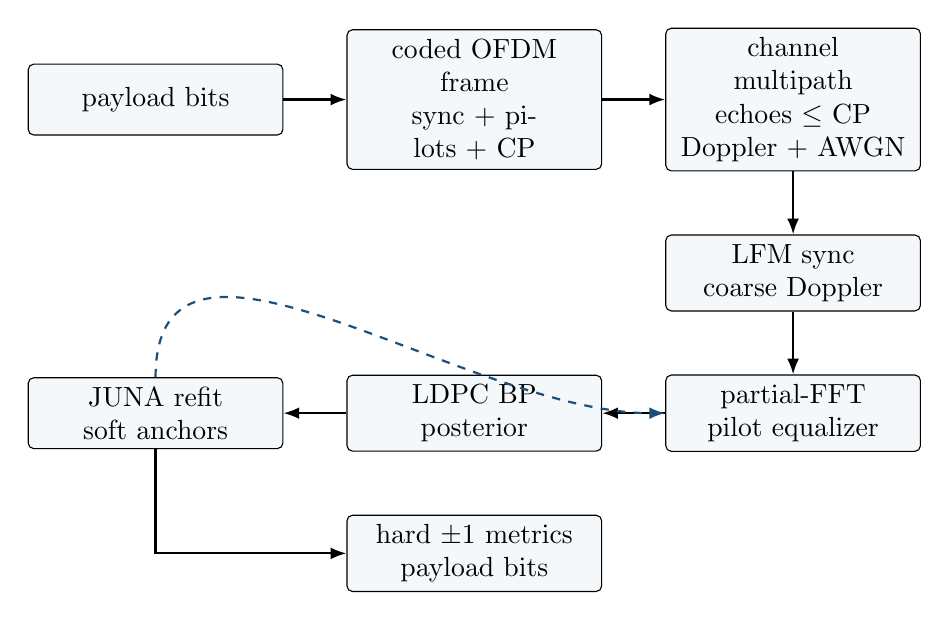
\begin{tikzpicture}[
  node distance=8mm,
  box/.style={draw, rounded corners=2pt, align=center, fill=softPanel,
              minimum height=9mm, text width=30mm},
  arr/.style={-{Latex[length=2mm]}, thick}
]
\node[box] (bits) {payload bits};
\node[box, right=of bits] (ofdm) {coded OFDM frame\\sync + pilots + CP};
\node[box, right=of ofdm] (chan) {channel\\multipath echoes \(\leq\) CP\\Doppler + AWGN};
\node[box, below=of chan] (sync) {LFM sync\\coarse Doppler};
\node[box, below=of sync] (pfft) {partial-FFT\\pilot equalizer};
\node[box, left=of pfft] (bp) {LDPC BP\\posterior};
\node[box, left=of bp] (refit) {\juna{} refit\\soft anchors};
\node[box, below=of bp] (out) {hard \(\pm 1\) metrics\\payload bits};
\draw[arr] (bits) -- (ofdm);
\draw[arr] (ofdm) -- (chan);
\draw[arr] (chan) -- (sync);
\draw[arr] (sync) -- (pfft);
\draw[arr] (pfft) -- (bp);
\draw[arr] (bp) -- (refit);
\draw[arr] (refit) |- (out);
\draw[arr, dashed, color=junaBlue] (refit.north) to[out=90,in=180] (pfft.west);
\end{tikzpicture}
\end{center}

Plain OFDM asks each carrier to stand mostly alone. Partial-FFT reception is
stronger: it windows the symbol in time and combines several views of each
carrier. A single full-length FFT assumes the channel holds still across the
whole symbol. Under Doppler it does not, so that one coefficient is a blurred
average; several FFTs, each over a shorter time window of the symbol, see less
motion and give the combiner (the weighted sum of these partial-FFT views)
something useful to fit.

\juna{} adds one more loop. After LDPC belief propagation, each data symbol has
a soft post-decoding estimate; high-confidence estimates behave most like
pilots. They are not new known tones transmitted over the channel; they are
decoder-supported guesses that help the receiver refit its combiner. The link
to pilots is the soft-pilot trick. A pilot works because the receiver already
knows the transmitted symbol,
so the distortion on that tone is a direct channel measurement. A data symbol
that the LDPC decoder returns with high confidence is almost as good as known,
so \juna{} treats it as a soft pilot and refits the equalizer against this
enlarged set of references. In the lite path, uncertainty is handled by
filtering the anchor set: low-confidence data tones are not reused as training
anchors. In the robust path, the update weights training by decoder confidence,
so unsure bits contribute less.

In communications terms this is an iterative decode-and-re-estimate loop,
closer to soft decision-directed channel estimation than to strict turbo
equalization. Rather than exchanging extrinsic LLRs with a soft-input
soft-output equalizer, \juna{} reuses posterior symbol means, dominated by the
confident tones, as soft pilots to re-fit its least-squares combiner.

\section{The Cost Behind Lite and Robust}

The code and older notes sometimes call the partial-FFT index a
\emph{branch}, but that word is overloaded in communications: it can mean an
antenna, a diversity path, or a channel tap. Here we use
\emph{partial-FFT view} for each receiver-side windowed FFT observation. After
the cyclic prefix is removed, the receiver cuts one OFDM symbol into \(P\)
nearly equal short-time windows. For each window it keeps that rectangular time
interval, zeros the rest of the symbol, and takes an \(N\)-point FFT. The result
\(y_{p,k}\) is the observation of tone \(k\) from partial-FFT view \(p\). The
combiner forms
\begin{equation}
  \hat{s}_k = \sum_{p=1}^{P} w_{p,b(k)}\,y_{p,k},
\end{equation}
where \(b(k)\) is a small frequency band and \(w_{p,b}\) is the view weight for
that band. Partial FFT is therefore a time-local view of the same OFDM symbol,
not a separate propagation path and not a change to the transmitted waveform.
Equivalently, for one tone,
\begin{equation}
  \mathbf y_k =
  \begin{bmatrix}
    y_{1,k}\\
    y_{2,k}\\
    \vdots\\
    y_{P,k}
  \end{bmatrix},
  \qquad
  \mathbf w_b =
  \begin{bmatrix}
    w_{1,b}\\
    w_{2,b}\\
    \vdots\\
    w_{P,b}
  \end{bmatrix},
  \qquad
  \hat{s}_k=\mathbf y_k^{\mathrm T}\mathbf w_{b(k)} .
\end{equation}
The lowercase bold symbol \(\mathbf w_b\) means one view-weight vector for band
\(b\). The capital bold symbol \(\mathbf W\) used below is the whole collection
of those vectors, one per band:
\(\mathbf W=\{\mathbf w_1,\ldots,\mathbf w_B\}\). They are the same kind of
combiner weight, but at different scopes.

Both \code{:lite} and \code{:robust} start from the same simple combiner-fit
problem. Suppose a set of tones \(T_b\) in band \(b\) has target symbols \(d_k\).
For pilots, \(d_k\) is known. After LDPC decoding, \(d_k\) can also be a
posterior-mean data symbol. In the lite update, low-confidence data tones are
left out of the anchor set; only tones above the confidence threshold, up to the
anchor cap, are reused as soft training targets. The combiner weights for that
band are fit by
\begin{equation}
  \min_{\mathbf w_b}\;
  \sum_{k\in T_b}\left|\sum_{p=1}^{P} w_{p,b}y_{p,k}-d_k\right|^2
  + \lambda_{\rm ridge}\|\mathbf w_b\|_2^2 .
\end{equation}
If \(T_b=\{k_1,\ldots,k_m\}\), the matrix form stacks the selected tones as
\begin{equation}
  Y_b =
  \begin{bmatrix}
    \mathbf y_{k_1}^{\mathrm T}\\
    \mathbf y_{k_2}^{\mathrm T}\\
    \vdots\\
    \mathbf y_{k_m}^{\mathrm T}
  \end{bmatrix}
  =
  \begin{bmatrix}
    y_{1,k_1} & y_{2,k_1} & \cdots & y_{P,k_1}\\
    y_{1,k_2} & y_{2,k_2} & \cdots & y_{P,k_2}\\
    \vdots & \vdots & \ddots & \vdots\\
    y_{1,k_m} & y_{2,k_m} & \cdots & y_{P,k_m}
  \end{bmatrix},
  \qquad
  \mathbf d_b =
  \begin{bmatrix}
    d_{k_1}\\
    d_{k_2}\\
    \vdots\\
    d_{k_m}
  \end{bmatrix}.
\end{equation}
Thus the fit is
\(\|Y_b\mathbf w_b-\mathbf d_b\|_2^2+
\lambda_{\rm ridge}\|\mathbf w_b\|_2^2\). Differentiating with
respect to \(\mathbf w_b^*\) and setting the result to zero gives
\begin{equation}
  (Y_b^{\mathrm{H}}Y_b+\lambda_{\rm ridge}I)\mathbf w_b
    = Y_b^{\mathrm{H}}\mathbf d_b ,
\end{equation}
which is the small normal equation solved in the code. That is the derivation
of the lite update. The receiver first seeds a partial-FFT plus FEC candidate; if
that candidate is already valid, it keeps it and skips the refit. Otherwise it
freezes the decoder posterior means as soft targets, chooses confident data
tones as additional anchors, refits the least-squares combiner, decodes again,
and keeps the better candidate. Lite can therefore be read as one
decision-directed block update of the combiner with the symbol beliefs held
fixed. It is not a gradient descent on every receiver variable.

\begin{algorithm}[t]
\caption{\juna{} lite posterior-anchor refit}
\begin{algorithmic}[1]
\Require Partial-FFT observations \(y_{p,k}\), pilots, LDPC decoder, anchor cap \(A_{\max}\)
\State Fit pilot-only combiners \(\mathbf W_0\) by ridge/RLS least squares
\State Decode the partial-FFT+FEC seed and record its validity, syndrome, score, and posterior confidence
\If{the seed is already acceptable}
  \State \Return the seed candidate
\EndIf
\State Freeze the decoder posterior means \(\widetilde d_k\) and confidences \(c_k\)
\For{each frequency band \(b\)}
  \State Select at most \(A_{\max}\) confident data tones in band \(b\)
  \State Stack pilots and selected data anchors into \(Y_b\) and \(\mathbf d_b\)
  \State Solve \((Y_b^{\mathrm H}Y_b+\lambda_{\rm ridge}I)\mathbf w_b
        =Y_b^{\mathrm H}\mathbf d_b\)
\EndFor
\State Equalize with the refit combiner collection \(\mathbf W\), then LDPC-decode again
\State \Return the better candidate under validity, syndrome, score, and posterior-confidence tests
\end{algorithmic}
\end{algorithm}

The robust mode is the gradient version of a richer, but still reduced, cost.
It keeps the full combiner collection \(\mathbf W\) as a variable and also lets
\(z\), a vector of LLR-like bit coordinates, move. These coordinates define
soft QPSK symbols through
\begin{equation}
  S_t(z)=\frac{1}{\sqrt{2}}\left[
    \tanh\!\left(\frac{z_{2t-1}}{2}\right)
    + j\,\tanh\!\left(\frac{z_{2t}}{2}\right)
  \right],
\end{equation}
with the second term omitted at the end if the codeword length is odd. In
the data-tie term, \(k_t\) is the tone that carries data symbol \(t\). The
channel response, Doppler time-scale, and timing are not variables in this
objective; they have already been folded into the partial-FFT observations
\(y_{p,k}\), the synchronization step, and the pilot fit \(\mathbf W_0\). Thus \(J\)
optimizes only the engineered receiver variables \(\mathbf W\) and \(z\), not a joint
physical-channel likelihood. The LDPC code constraints are fixed; they enter as
a parity penalty on \(z\), and they influence \(\mathbf W\) only through the
data-tie term that couples \(\hat{s}_{k_t}(\mathbf W)\) to \(S_t(z)\). For
readability, the coefficients below absorb the implementation's per-count
normalizations over pilots, data tones, checks, and variables:
\begin{equation}
\begin{aligned}
J(\mathbf W,z) ={}&
  \alpha\sum_{\text{pilots}}\left|\hat{s}_k(\mathbf W)-p_k\right|^2
  + \beta\sum_{\text{data }t} c_t
      \left|\hat{s}_{k_t}(\mathbf W)-S_t(z)\right|^2 \\
&+ \lambda\sum_{\text{checks}}
      \left(1-\prod_{i\in\text{check}}\tanh(z_i/2)\right)^2
  + \eta\|\mathbf W-\mathbf W_0\|^2
  + \mu\|z-z_0\|^2
  + \gamma\|z\|^2 .
\end{aligned}
\end{equation}
The first term keeps known pilots matched. The second ties equalized data tones
to the current soft symbols, weighted by decoder confidence \(c_t\), computed
once from the BP-seed posterior \(z_0\) and then held fixed during the Adam
updates. The third is a smooth LDPC parity-check penalty: \(\tanh(z_i/2)\) is
the soft \(\pm1\) value of bit \(i\), and a satisfied parity check has product
\(+1\), so this term penalizes a soft check product that drifts away from
satisfaction. The \(\eta\) and \(\mu\) terms keep the combiner near the pilot
fit \(\mathbf W_0\) and the LLR coordinates near the BP seed \(z_0\). The final
\(\gamma\|z\|^2\) term is a plain ridge that shrinks undecided LLR coordinates
toward zero. Together these regularizers stop the optimizer from drifting far
from the pilot-fit and BP-seed starting point. Unlike lite, robust has no
closed-form update; \(J(\mathbf W,z)\) is a hand-built reduced objective, and the code
descends its gradients with Adam. The receiver decodes a candidate at each step
and keeps the best decoded candidate under validity, syndrome, score, and
mean-absolute-posterior tests.

\begin{algorithm}[t]
\caption{\juna{} robust reduced gradient refinement}
\begin{algorithmic}[1]
\Require Seed \((\mathbf W_0,z_0)\), fixed confidences \(c_t\), fixed LDPC checks, step budget \(G\)
\State Initialize \(\mathbf W\gets\mathbf W_0\), \(z\gets z_0\), and best candidate from the seed decode
\For{\(g=1,\ldots,G\)}
  \State Form soft symbols \(S_t(z)\)
  \State Evaluate \(J(\mathbf W,z)\) from Eq.~(7)
  \State Compute gradients \(\nabla_{\mathbf W}J\) and \(\nabla_zJ\)
  \State Take one Adam step on \(\mathbf W\) and \(z\)
  \State Equalize with the updated \(\mathbf W\), map \(z\) to LLRs, and LDPC-decode a checkpoint
  \State Keep the best checkpoint under validity, syndrome, score, and posterior-confidence tests
\EndFor
\State \Return the best decoded candidate
\end{algorithmic}
\end{algorithm}

\begin{figure}[t]
\centering
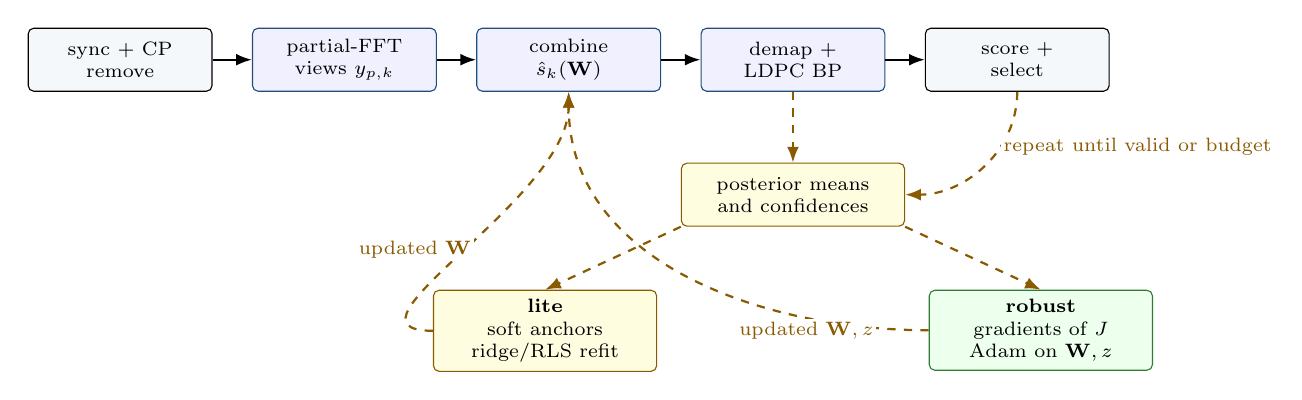
\begin{tikzpicture}[
  >=Latex,
  font=\scriptsize,
  node distance=7mm and 5mm,
  stage/.style={draw, rounded corners=2pt, align=center, fill=softPanel,
                minimum height=8mm, text width=21mm},
  loopstage/.style={draw=junaBlue, rounded corners=2pt, align=center,
                    fill=blue!6, minimum height=8mm, text width=21mm},
  feedbackbox/.style={draw=junaGold, rounded corners=2pt, align=center,
                      fill=yellow!12, minimum height=8mm, text width=26mm},
  gradbox/.style={draw=junaGreen, rounded corners=2pt, align=center,
                  fill=green!7, minimum height=8mm, text width=26mm},
  tag/.style={fill=white, inner sep=1pt},
  arr/.style={-{Latex[length=2mm]}, thick},
  looparr/.style={-{Latex[length=2mm]}, thick, dashed, color=junaGold}
]
\node[stage] (sync) {sync + CP\\remove};
\node[loopstage, right=of sync] (pfft) {partial-FFT\\views \(y_{p,k}\)};
\node[loopstage, right=of pfft] (eq) {combine\\\(\hat{s}_k(\mathbf W)\)};
\node[loopstage, right=of eq] (bp) {demap +\\LDPC BP};
\node[stage, right=of bp] (select) {score +\\select};

\draw[arr] (sync) -- (pfft);
\draw[arr] (pfft) -- (eq);
\draw[arr] (eq) -- (bp);
\draw[arr] (bp) -- (select);

\node[feedbackbox, below=9mm of bp] (post) {posterior means\\and confidences};
\node[feedbackbox, below left=8mm and 3mm of post] (lite) {\textbf{lite}\\soft anchors\\ridge/RLS refit};
\node[gradbox, below right=8mm and 3mm of post] (robust) {\textbf{robust}\\gradients of \(J\)\\Adam on \(\mathbf W,z\)};

\draw[looparr] (bp.south) -- (post.north);
\draw[looparr] (post.south west) -- (lite.north);
\draw[looparr] (post.south east) -- (robust.north);
\draw[looparr] (lite.west) to[out=180,in=-90] node[pos=0.55,below left,tag] {updated \(\mathbf W\)}
  (eq.south);
\draw[looparr] (robust.west) to[out=180,in=-90] node[pos=0.24,below,tag] {updated \(\mathbf W,z\)}
  (eq.south);
\draw[looparr] (select.south) to[out=-90,in=0] node[pos=0.35,right,tag] {repeat until valid or budget}
  (post.east);
\end{tikzpicture}
\caption{Pictorial view of the \juna{} feedback loop. The top row is the seed
receiver path. The dashed loop is the decoder-to-equalizer feedback inspired by
the slide deck: LDPC posteriors either become soft anchors for a lite
least-squares refit or drive a robust gradient step, after which the receiver
equalizes and decodes another candidate.}
\end{figure}

So the hierarchy is:
\begin{itemize}
  \item \code{:lite}: closed-form least-squares refit with posterior symbols
        held fixed as soft targets;
  \item \code{:robust}: gradient descent on the reduced \(\mathbf W,z\) objective, where
        combiner weights and soft symbol LLR coordinates move together.
\end{itemize}

Calling \code{:robust} ``complete'' is only safe in this limited sense: it is the
complete implemented cost for the reduced \(\mathbf W,z\) receiver path, meaning the
variables it actually moves are the combiner weights and the soft code-symbol
LLR coordinates. It is not a full physical-channel likelihood, not a
timing/acquisition
optimizer, and not a joint estimator over passband propagation, Doppler
trajectory, carrier phase, sample timing, synchronization, and codeword.

\section{The Local Demo as a First Experiment}

The first step is a one-time environment setup:
\begin{verbatim}
julia --project=. -e 'using Pkg; Pkg.instantiate()'
\end{verbatim}

Run these commands from inside the \code{Juna/} folder. That environment step is
needed once on a fresh checkout. The LDPC helper tools
\code{make-ldpc}, \code{make-gen}, and \code{print-pchk} must also be available
on \code{PATH} or beside \code{LDPC.jl}; they are platform-specific binaries and
are not committed in this folder. Without them, code construction fails with a
\code{could not spawn make-ldpc} error. With the environment and LDPC tools in
place, the first actual experiment is:
\begin{verbatim}
julia --project=. demo_isi_ici_awgn.jl
\end{verbatim}

In the current folder, one seeded run prints:
\begin{verbatim}
channel: 4-tap multipath (max delay 142 <= CP 256)
         + Doppler a=1.0015 + AWGN 20 dB
lite   : a_est=1.00145  (cfo=+34.88 Hz)  BER = 0/1024 = 0.000e+00
robust : a_est=1.00145  (cfo=+34.88 Hz)  BER = 0/1024 = 0.000e+00
\end{verbatim}
\noindent\emph{Transcript note: the program prints the channel description on
one line; it is wrapped here to fit the page. The program also prints a Unicode
less-than-or-equal sign where this transcript uses \code{<=}.}

This small printout teaches several ideas at once:
\begin{itemize}
  \item \textbf{The echoes fit inside the CP.} The 142-sample maximum excess
        delay is shorter than the 256-sample cyclic prefix, so the synthetic
        echo tail does not spill into the next block; each tone is mainly left
        with a frequency-selective complex gain. Because the sync removes the
        bulk time-scale, the residual Doppler-induced ICI in this run is small
        and the pilot equalizer, combiner, and LDPC clean it up comfortably at
        20 dB.
  \item \textbf{Doppler is present.} The waveform is time-scaled by
        \code{a=1.0015}; the sync estimates it as about \code{1.00145}. The
        receiver reports this through the \code{cfo} field as
        \((a_{\mathrm{est}}-1)f_c\), so the rounded value
        \((1.00145-1)\times24\,\mathrm{kHz}\) gives about \(+34.8\) Hz; the
        transcript's \(+34.88\) Hz uses the unrounded estimate. Here the
        positive sign follows the code's time-scale convention, positive for
        \(a>1\), not a signed physical carrier shift. The underlying time-scale
        shifts each tone by an amount proportional to its frequency, so a single
        carrier offset cannot fully describe it. At a 1500 m/s sound speed, that
        scale is roughly 2.2 m/s of relative motion.
  \item \textbf{The channel is at a favorable noise level.} AWGN is added at a 20 dB
        signal-to-noise ratio; higher dB means less noise, and this favorable
        level is part of why both modes decode this frame cleanly.
  \item \textbf{Both receiver modes succeed on this realization.} The demo is
        not a proof of universal performance; it is a compact sanity check.
\end{itemize}

\section{Lite and Robust Modes}

The same modulation object has two receiver modes:
\begin{center}
\begin{tabular}{p{0.16\linewidth}p{0.42\linewidth}p{0.30\linewidth}}
\toprule
Mode & Mechanism & Teaching interpretation \\
\midrule
\code{:lite} & post-decoding anchor least-squares refit & fast decoder feedback via soft anchors \\
\code{:robust} & reduced gradient over combiner and symbol estimates & higher-cost path for harder ICI \\
\bottomrule
\end{tabular}
\end{center}

For a newcomer, the key idea is not the specific solver; it is that both modes
use decoder information before giving up on the equalizer.
\code{:lite} is the first one to teach because it has the cleanest mental model:
trusted decoded symbols become soft anchors.

\section{What the UnetStack Bench Adds}

The \code{bench/} folder contributes a second beginner paper angle: \juna{} is
not just an isolated simulation. It can be explained as a modem that fits a
larger acoustic networking stack.

Here ``Yoda-style OFDM'' concretely means \code{bench/OFDM\_musique.jl}, a
Julia clean-room reference for the Yoda \code{ofdm} waveform. Deployed Yoda
itself is a closed Java/native stack that this folder does not run against.

The file \code{bench/explain\_juna\_yoda\_sim.jl} teaches three boundaries:
\begin{enumerate}
  \item the \code{musique} OFDM reference and \juna{} can share the same Julia
        modulation API;
  \item \juna{} can ride a Yoda-shaped baseband path of interleaved complex
        samples;
  \item sharing an interface does not mean the Yoda-style OFDM receiver in the
        \code{musique} reference can decode \juna{} waveforms, or vice versa.
\end{enumerate}

That is a useful newbie distinction. ``Compatible with the stack'' means the
objects have the same service shape. It does not mean the two waveforms are
bit-compatible.

\section{Honest Limits}

Six facts this demo does not establish:
\begin{itemize}
  \item The demo does not prove measured-channel performance.
  \item It does not show that \juna{} is the same waveform as Yoda OFDM.
  \item It does not show that the robust mode always beats the lite mode.
  \item It does not net out pilot, FEC, CP, or sync overhead.
  \item Its 20 dB number is a per-sample complex-baseband SNR, not an
        \(E_b/N_0\) point for a rate-matched BER curve.
  \item It runs at complex baseband and starts from an isolated captured frame;
        it skips passband up/down-conversion, AGC, fine timing, and detecting
        the frame inside a continuous noisy stream. The LFM sync provides coarse
        frame alignment and Doppler, not a full deployed receiver front end.
\end{itemize}

The right claim is more modest and more useful: this folder gives a runnable,
minimal ladder for understanding \juna{} from the interface upward.

\section{Takeaway}

The strongest beginner explanation is not ``\juna{} is a better OFDM.'' It is:

\begin{quote}
\juna{} is what happens when an OFDM receiver stops treating the decoder as the
last step and starts treating it as a source of soft evidence for the equalizer.
\end{quote}

\end{document}
